\chapter{Overview}\label{s:overview}
This overview contains a Utility Tree, which captures the Architecturally significant requirements (ASR). These ASRs are extracted from the Business Goals and Concerns of stakeholders. Definition of these sources can be read in Appendix A.

\graphicspath{ {./images/} }
\begin{figure}[t]
\centering
\caption{Decomposition of Architecturally significant requirements}
\label{fig:mesh1}
\end{figure}

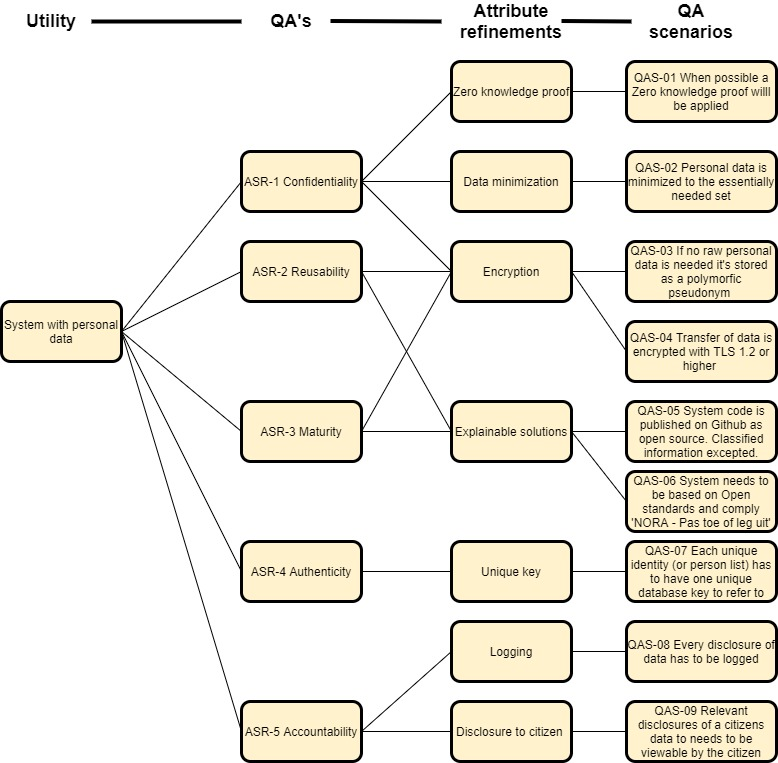
\includegraphics[width=14cm]{Decomposition of ASR and QAS.jpg}



\begin{tabular}{ |p{3cm}||p{10cm}|}
 \hline
 \multicolumn{2}{|l|}{Business goal 1 - Explainable solutions} \\
 \hline
 Shorthand name   & BG-1 Explainable solutions    \\
 \hline
 Description &   Communicate simple how technology works to raise awareness and support. Also, provide more detailed scientific information for experts to contribute as a community.  \\
  \hline
 Stakeholders involved & Interviewee 3 - Directing architect  \\
  \hline
 Quality Requirements   & QA-xx, QA-xx, QA-xx, QA-xx \\
  \hline
 Concerns &   C-xx, C-xx, C-xx, C-xx, C-xx\\
  \hline
 Fitting this into Business Goal Scenario & AD \\
 \hline
\end{tabular}


\todo{
This section provides a high-level outline of the proposed system or solution.
It typically illustrates the system architecture or the interactions between the
different solution components (via a “boxes-and-arrows” diagram) from a user’s
perspective.
}